\documentclass[]{article}
\usepackage{lmodern}
\usepackage{amssymb,amsmath}
\usepackage{ifxetex,ifluatex}
\usepackage{fixltx2e} % provides \textsubscript
\ifnum 0\ifxetex 1\fi\ifluatex 1\fi=0 % if pdftex
  \usepackage[T1]{fontenc}
  \usepackage[utf8]{inputenc}
\else % if luatex or xelatex
  \ifxetex
    \usepackage{mathspec}
  \else
    \usepackage{fontspec}
  \fi
  \defaultfontfeatures{Ligatures=TeX,Scale=MatchLowercase}
\fi
% use upquote if available, for straight quotes in verbatim environments
\IfFileExists{upquote.sty}{\usepackage{upquote}}{}
% use microtype if available
\IfFileExists{microtype.sty}{%
\usepackage{microtype}
\UseMicrotypeSet[protrusion]{basicmath} % disable protrusion for tt fonts
}{}
\usepackage[margin=1in]{geometry}
\usepackage{hyperref}
\hypersetup{unicode=true,
            pdftitle={Appendix A: Supplemental Methods},
            pdfauthor={Tim M. Szewczyk, Marek Petrik, Jenica M. Allen},
            pdfborder={0 0 0},
            breaklinks=true}
\urlstyle{same}  % don't use monospace font for urls
\usepackage{color}
\usepackage{fancyvrb}
\newcommand{\VerbBar}{|}
\newcommand{\VERB}{\Verb[commandchars=\\\{\}]}
\DefineVerbatimEnvironment{Highlighting}{Verbatim}{commandchars=\\\{\}}
% Add ',fontsize=\small' for more characters per line
\usepackage{framed}
\definecolor{shadecolor}{RGB}{248,248,248}
\newenvironment{Shaded}{\begin{snugshade}}{\end{snugshade}}
\newcommand{\AlertTok}[1]{\textcolor[rgb]{0.94,0.16,0.16}{#1}}
\newcommand{\AnnotationTok}[1]{\textcolor[rgb]{0.56,0.35,0.01}{\textbf{\textit{#1}}}}
\newcommand{\AttributeTok}[1]{\textcolor[rgb]{0.77,0.63,0.00}{#1}}
\newcommand{\BaseNTok}[1]{\textcolor[rgb]{0.00,0.00,0.81}{#1}}
\newcommand{\BuiltInTok}[1]{#1}
\newcommand{\CharTok}[1]{\textcolor[rgb]{0.31,0.60,0.02}{#1}}
\newcommand{\CommentTok}[1]{\textcolor[rgb]{0.56,0.35,0.01}{\textit{#1}}}
\newcommand{\CommentVarTok}[1]{\textcolor[rgb]{0.56,0.35,0.01}{\textbf{\textit{#1}}}}
\newcommand{\ConstantTok}[1]{\textcolor[rgb]{0.00,0.00,0.00}{#1}}
\newcommand{\ControlFlowTok}[1]{\textcolor[rgb]{0.13,0.29,0.53}{\textbf{#1}}}
\newcommand{\DataTypeTok}[1]{\textcolor[rgb]{0.13,0.29,0.53}{#1}}
\newcommand{\DecValTok}[1]{\textcolor[rgb]{0.00,0.00,0.81}{#1}}
\newcommand{\DocumentationTok}[1]{\textcolor[rgb]{0.56,0.35,0.01}{\textbf{\textit{#1}}}}
\newcommand{\ErrorTok}[1]{\textcolor[rgb]{0.64,0.00,0.00}{\textbf{#1}}}
\newcommand{\ExtensionTok}[1]{#1}
\newcommand{\FloatTok}[1]{\textcolor[rgb]{0.00,0.00,0.81}{#1}}
\newcommand{\FunctionTok}[1]{\textcolor[rgb]{0.00,0.00,0.00}{#1}}
\newcommand{\ImportTok}[1]{#1}
\newcommand{\InformationTok}[1]{\textcolor[rgb]{0.56,0.35,0.01}{\textbf{\textit{#1}}}}
\newcommand{\KeywordTok}[1]{\textcolor[rgb]{0.13,0.29,0.53}{\textbf{#1}}}
\newcommand{\NormalTok}[1]{#1}
\newcommand{\OperatorTok}[1]{\textcolor[rgb]{0.81,0.36,0.00}{\textbf{#1}}}
\newcommand{\OtherTok}[1]{\textcolor[rgb]{0.56,0.35,0.01}{#1}}
\newcommand{\PreprocessorTok}[1]{\textcolor[rgb]{0.56,0.35,0.01}{\textit{#1}}}
\newcommand{\RegionMarkerTok}[1]{#1}
\newcommand{\SpecialCharTok}[1]{\textcolor[rgb]{0.00,0.00,0.00}{#1}}
\newcommand{\SpecialStringTok}[1]{\textcolor[rgb]{0.31,0.60,0.02}{#1}}
\newcommand{\StringTok}[1]{\textcolor[rgb]{0.31,0.60,0.02}{#1}}
\newcommand{\VariableTok}[1]{\textcolor[rgb]{0.00,0.00,0.00}{#1}}
\newcommand{\VerbatimStringTok}[1]{\textcolor[rgb]{0.31,0.60,0.02}{#1}}
\newcommand{\WarningTok}[1]{\textcolor[rgb]{0.56,0.35,0.01}{\textbf{\textit{#1}}}}
\usepackage{graphicx,grffile}
\makeatletter
\def\maxwidth{\ifdim\Gin@nat@width>\linewidth\linewidth\else\Gin@nat@width\fi}
\def\maxheight{\ifdim\Gin@nat@height>\textheight\textheight\else\Gin@nat@height\fi}
\makeatother
% Scale images if necessary, so that they will not overflow the page
% margins by default, and it is still possible to overwrite the defaults
% using explicit options in \includegraphics[width, height, ...]{}
\setkeys{Gin}{width=\maxwidth,height=\maxheight,keepaspectratio}
\IfFileExists{parskip.sty}{%
\usepackage{parskip}
}{% else
\setlength{\parindent}{0pt}
\setlength{\parskip}{6pt plus 2pt minus 1pt}
}
\setlength{\emergencystretch}{3em}  % prevent overfull lines
\providecommand{\tightlist}{%
  \setlength{\itemsep}{0pt}\setlength{\parskip}{0pt}}
\setcounter{secnumdepth}{5}
% Redefines (sub)paragraphs to behave more like sections
\ifx\paragraph\undefined\else
\let\oldparagraph\paragraph
\renewcommand{\paragraph}[1]{\oldparagraph{#1}\mbox{}}
\fi
\ifx\subparagraph\undefined\else
\let\oldsubparagraph\subparagraph
\renewcommand{\subparagraph}[1]{\oldsubparagraph{#1}\mbox{}}
\fi

%%% Use protect on footnotes to avoid problems with footnotes in titles
\let\rmarkdownfootnote\footnote%
\def\footnote{\protect\rmarkdownfootnote}

%%% Change title format to be more compact
\usepackage{titling}

% Create subtitle command for use in maketitle
\providecommand{\subtitle}[1]{
  \posttitle{
    \begin{center}\large#1\end{center}
    }
}

\setlength{\droptitle}{-2em}

  \title{Appendix A: Supplemental Methods}
    \pretitle{\vspace{\droptitle}\centering\huge}
  \posttitle{\par}
  \subtitle{The performance of presence-based and process-based species distribution
models under realistic conditions}
  \author{Tim M. Szewczyk, Marek Petrik, Jenica M. Allen}
    \preauthor{\centering\large\emph}
  \postauthor{\par}
    \date{}
    \predate{}\postdate{}
  
\newcommand{\beginsupplement}{\setcounter{table}{0}  \renewcommand{\thetable}{A.\arabic{table}} \setcounter{figure}{0} \renewcommand{\thefigure}{A.\arabic{figure}}}  \usepackage{longtable}  \usepackage{caption}

\begin{document}
\maketitle

{
\setcounter{tocdepth}{1}
\tableofcontents
}
\setcounter{table}{0}  \renewcommand{\thetable}{A.\arabic{table}} \setcounter{figure}{0} \renewcommand{\thefigure}{A.\arabic{figure}}

\begin{center}\rule{0.5\linewidth}{\linethickness}\end{center}

This appendix contains supplemental methods pertaining to the virtual
species, species distribution models, and scenarios.

\begin{center}\rule{0.5\linewidth}{\linethickness}\end{center}

\section{Integral Projection Model structure}
\subsection{Overview}

To generate fully-known true distributions for the virtual species, we
used the general structure of an Integral Projection Model (IPM) to
calculate the intrinsic growth rate \(\lambda\) in each cell of the
gridded landscape, and adapted the regression-based structure of an IPM
into an individual-level, simulation-based cellular automata (CA) model
to produce spatiotemporally dynamic abundance distributions.

IPMs (Easterling 2000; Merow et al.~2014, 2017) use the size
distribution, \(z\), of individuals at time \(t\), along with a kernel
\(K(z^{\prime}, z)\), to predict the size distribution, \(z^{\prime}\),
at time \(t+1\): \begin{equation}
n_{t+1}(z^{\prime}) = \int_{\Omega} K(z^{\prime}, z) n_t(z) dz
\end{equation}

Here, \(\Omega\) represents the range of possible sizes for the species
or population. The kernel \(K(z^{\prime}, z)\) is composed of a growth
and survival component, \(P(z, z^{\prime})\), representing the fate of
individuals from time \(t\) to \(t+1\), and a fecundity component,
\(F(z, z^{\prime})\), representing new individuals added between time
\(t\) and \(t+1\). In practice, the integral is approximated using a
discretized transition matrix, and the intrinsic growth rate \(\lambda\)
is calculated as the first eigenvalue of the transition matrix.

The \(P\) and \(F\) kernels are decomposed further into more mechanistic
conditional probabilities and parameters, many of which are functions of
the size distribution \(z\). For example: \begin{equation}
\begin{split}
K(z^{\prime}, z) & = P(z^{\prime}, z) + F(z^{\prime}, z) \\
    & = s(z) g(z^{\prime}|z) + p_{flower}(z) f_{seeds}(z) p_{estab} f_{rcrSize}(z^{\prime})
\end{split}
\end{equation}

where \(s(z)\) is the survival probability of individuals based on size,
\(g(z^{\prime}|z)\) is the probability density of size \(z^{\prime}\)
for an individual of size \(z\), \(p_{flower}(z)\) is the probability
that an individual of size \(z\) produces flowers, \(f_{seeds}(z)\) is
the expected number of seeds produced by an individual of size \(z\)
given that they flower, \(p_{estab}\) is the probability that a seed
germinates and establishes as a new recruit, and
\(f_{rcrSize}(z^{\prime})\) is the expected size distribution of new
recruits at time \(t+1\). On a gridded landscape, the population in each
cell could be modelled independently using the above structure, with
environmental effects incorporated by allowing the environment to
influence parameter values (e.g., \(f_{seeds}\)).

\subsection{Adding a seed bank}

This basic IPM structure is very flexible, allowing for discrete life
stages, reproduction-dependent mortality, and environmental covariates.
To incorporate a seed bank where seeds that do not germinate between
time \(t\) and \(t+1\) may survive to \(t+2\) or beyond, the fecundity
kernel is altered, with seed bank \(B\), such that: \begin{align}
n_{t+1}(z^{\prime}) &= B_t s_{rcrB} p_{estab} f_{rcrSize}(z^{\prime}) + \int_{\Omega}[P(z^{\prime}, z)+F(z^{\prime}, z)] n_t(z) dz \\
F(z^{\prime}, z) &= p_{flower}(z)  f_{seeds}(z) s_{rcrDirect} p_{estab} f_{rcrSize}(z^{\prime}) \\
B_{t+1} &= B_t s_{survB} (1-s_{rcrB})  + p_{flower}(z)  f_{seeds}(z) (1-s_{rcrDirect}) s_{survB} n_t(z) dz
\end{align}

where \(B_t\) is the number of seeds in the seed bank at time \(t\),
\(s_{rcrB}\) is the probability a seed recruits from the seed bank,
\(s_{survB}\) is the probability a seed survives in the seed bank from
time \(t\) to \(t+1\), and \(s_{rcrDirect}\) is the probability a seed
produced in year \(t\) germinates between year \(t\) and \(t+1\). Two
notes about the structure and definitions: 1) a seed added to the seed
bank must fail to recruit in time \(t\) and must also survive from \(t\)
to \(t+1\), and 2) the probability of recruiting is best interpreted as
the probability of germinating and is therefore separate from the
probability of establishing. Both of these could be defined differently
to combine each set of processes, though keeping them separate allows
for seeds to perish.

\subsection{Adding dispersal}

The above equations assume isolated populations in each cell. However,
for a typical plant species, dispersal occurs when seeds move from the
cell where they are produced to a different cell. In an IPM with a seed
bank, this will affect the fecundity kernel \(F(z^{\prime}, z)\) and the
seed bank \(B\). Specifically, the number of seeds in the seed bank in
cell \(i\) at time \(t+1\) will be the number of seeds surviving in the
seed bank \(B_i\) from time \(t\) to \(t+1\), plus the number of seeds
produced in cell \(i\) at time \(t\) that remain in cell \(i\) and do
not recruit directly, plus the number of seeds entering cell \(i\) from
cells \(j = 1, ..., J\) as immigrants in time \(t\) that then fail to
recruit directly: \begin{equation}
    \begin{aligned}
        B_{i,t+1} = \enspace
        & B_{i,t} s_{survSB} (1-s_{rcrSB}) \enspace+  \\
        & \int_{\Omega} p_{flower,i}(z)  f_{seeds,i}(z) (1-p_{emig}) (1-s_{rcrDirect}) s_{survB} n_{i,t}(z) dz \enspace+  \\
        & \sum_{j=1}^{J} \int_{\Omega} [p_{flower,j}(z)  f_{seeds,j}(z) p_{emig} n_{t,j}(z) dz] p_{SDD,ji} (1-s_{rcrDirect}) s_{survB}\\
    \end{aligned}
\end{equation} \begin{equation}
\begin{aligned}
n_{i,t+1}(z^{\prime}) = \enspace
& B_{i,t} s_{rcrSB} p_{estab_i} f_{rcrSize}(z^{\prime}) \enspace+   \\
& \int_{\Omega} [s_i(z) g_i(z^{\prime}|z) + p_{flower_i}(z)  f_{seeds_i}(z) (1-p_{emig}) s_{rcrDirect} p_{estab_i} f_{rcrSize}(z^{\prime})] n_{i,t}(z) dz \enspace +  \\
& \sum_{j=1}^{J} \int_{\Omega} [p_{flower,j}(z)  f_{seeds,j}(z) p_{emig} n_{t, j}(z) dz] p_{SDD,ji} s_{rcrDirect} p_{estab,i} f_{rcrSize}(z^{\prime})\\
\end{aligned}
\end{equation} for each cell \(i\) which is a target cell of each cell
\(j\) of \(J\) cells, where the integral describes the seed production
in each cell \(j\) and \(p_{SDD,ji}\) is the probability that a seed
dispersed from \(j\) lands in \(i\). Note that, as above, seeds added to
the seed bank must survive overwinter as well as fail to recruit
directly.

\begin{center}\rule{0.5\linewidth}{\linethickness}\end{center}

\newpage
\section{Virtual species simulation}

We used the above IPM structure, including a seed bank and dispersal, as
the basis for the virtual species. Thus, the population in each cell
\(i\) has size distribution \(z\), where \(z^{\prime}\) is the size
distribution the next year, and \(\boldsymbol{z_i}\) is a matrix with
columns of 1 (intercept) and \(z\). For the IPMs, we used the following
regression equations to populate discretized transition matrices for
each cell to then calculate the deterministic intrinsic growth rate
\(\lambda\). For the CA\textsubscript{i} models, we used the same
regression equations to generate expected values for each individual,
and then drew simulated outcomes from the specified distribtutions.

\subsection{Survival}

Annual survival, \(\boldsymbol{s_i}\), was modelled for each individual
in cell \(i\) as a binary outcome (0: mortality; 1: survival) following
a Bernoulli distribution with probability \(\boldsymbol{\psi_{si}}\)
such that: \begin{align}
\boldsymbol{s_i} & \sim Bern(\boldsymbol{\psi_{si}}) \\
logit(\boldsymbol{\psi_{si}}) & = \boldsymbol{z_i}\beta_{s} + \boldsymbol{X_i}\theta_{s}
\end{align} where \(\beta_{s}\) is a vector of covariates for size,
\(\boldsymbol{X_i}\) is a set of cell-level environmental covariates,
and \(\theta_{s}\) is a vector of responses to the environmental
covariates.

\subsection{Growth}

The size distribution, \(\boldsymbol{z^{\prime}_i}\) of individuals in
cell \(i\) for time \(t+1\) was distributed normally about the vector of
expected sizes, \(\boldsymbol{\mu_{gi}}\) with standard deviation
\(\sigma_g\), such that \begin{align}
\boldsymbol{z^{\prime}_i} &\sim Norm(\boldsymbol{\mu_{gi}}, \sigma_g) \\
\boldsymbol{\mu_{gi}} &= \boldsymbol{z_i}\beta_{g} + \boldsymbol{X_i}\theta_{g}
\end{align} where \(\beta_{g}\) is a vector of covariates for size,
\(\boldsymbol{X_i}\) is a set of cell-level environmental covariates,
and \(\theta_{g}\) is a vector of responses to the environmental
covariates.

\subsection{Flowering}

Individual flowering, \(\boldsymbol{l_i}\), was modelled for each
individual in cell \(i\) as a binary outcome (0: no flowers; 1: flowers)
following a Bernoulli distribution with probability
\(\boldsymbol{\psi_{li}}\) such that: \begin{align}
\boldsymbol{l_i} &\sim Bern(\boldsymbol{\psi_{li}}) \\
logit(\boldsymbol{\psi_{li}}) &= \boldsymbol{z_i}\beta_{l} + \boldsymbol{X_i}\theta_{l}
\end{align} where \(\beta_{l}\) is a vector of covariates for size,
\(\boldsymbol{X_i}\) is a set of cell-level environmental covariates,
and \(\theta_{l}\) is a vector of responses to the environmental
covariates.

\subsection{Seeds}

The number of seeds produced, \(\boldsymbol{d_i}\) by each flowering
individual in cell \(i\) for time \(t\) was Poisson distributed about
the vector of expected seed counts, \(\boldsymbol{\mu_{di}}\), such that
\begin{align}
\boldsymbol{d_i} &\sim Poisson(\boldsymbol{\mu_{di}}) \\
log(\boldsymbol{\mu_{di}}) &= \boldsymbol{z_i}\beta_{d} + \boldsymbol{X_i}\theta_{d}
\end{align} where \(\beta_{d}\) is a vector of covariates for size,
\(\boldsymbol{X_i}\) is a set of cell-level environmental covariates,
and \(\theta_{d}\) is a vector of responses to the environmental
covariates. In each cell \(i\), the seeds produced stay in the cell,
emigrate through short distance dispersal, or perish. Seeds that survive
may either enter the seed bank or recruit directly.

\subsection{Dispersal}

The total number of immigrant seeds arriving in a cell, \(D_i\) is
calculated as the sum of the seeds from nearby cells that disperse from
cell \(j\) to cell \(i\), such that: \begin{equation}
D_i = \sum\limits_{j=1}^J \sum\limits_{n=1}^{N_j} \boldsymbol{d_j}p_{emig}p_{ji}
\end{equation} where \(J\) is the number of cells dispersing into \(i\),
\(N_j\) is the number of individuals in cell \(j\), \(d_j\) is the
vector of seed numbers produced by individuals in cell \(j\),
\(p_{emig}\) is the probability that seeds produced in cell \(j\)
emigrate, and \(p_{ji}\) is the probability that a seed emigrating from
cell \(j\) is dispersed to cell \(i\).

\subsection{Recruits}

The number of recruits, \(n_{rcr,i}\) in cell \(i\) in time \(t\), may
originate either from the seed bank, from seeds produced in cell \(i\)
in year \(t\), or from immigrant seeds arriving in year \(t\), such
that: \begin{align}
n_{rcr,i} &= B_i p_{rcrB}p_{est} + \sum\limits_{n=1}^{N_i} \boldsymbol{d_i}(1-p_{emig})p_{rcrDirect}p_{est} + D_i p_{rcrDirect}p_{est}\\
\boldsymbol{z^{\prime}_{rcr,i}} &\sim Norm(\mu_{rcr.z}, \sigma_{rcr.z})
\end{align} where \(B_i\) is the number of seeds in the seed bank,
\(p_{rcrB}\) is the probability that a seed germinates from the seed
bank, \(p_{est}\) is the probability that a new seedling establishes,
\(p_rcrDirect\) is the probability that a seed germinates in the year it
was produced, \(z^{\prime}_{rcr,i}\) is the size distribution of new
recruits in year \(t+1\), \(\mu_{rcr.z}\) is the mean recruit size, and
\(\sigma_{rcr.z}\) is the standard deviation of recruit size.

\subsection{Seed Bank}

Finally, the seed bank for year \(t+1\) is calculated as the sum of the
seeds remaining in the seed bank, the seeds produced in cell \(i\) and
entering into the seed bank, and the immigrant seeds entering into the
seed bank, such that: \begin{equation}
B^{\prime}_i = B_i(1-p_{rcrB})s_B + \sum\limits_{n=1}^{N_i} \boldsymbol{d_i}(1-p_{emig})(1-p_{rcrDirect})s_B + D_i(1-p_{rcrDirect})s_B
\end{equation} where \(s_B\) is the probability that a seed survives in
the seed bank to the next year.

\begin{center}\rule{0.5\linewidth}{\linethickness}\end{center}

\newpage
\section{Species Distribution Model details}

This section of the appendix contains additional information regarding
the structure of the species distribution models. The full R code is
available from \url{https://github.com/Sz-Tim/sdmMethodComp}.

\subsection{IPM}

The Integral Projection Models for each species followed the structure
described in the previous section. For each dataset (100 datasets x 2
species x 4 data scenarios), we fit regressions for each vital rate
regression using the R package \emph{MuMIn} to compare all combinations
of climatic variables. The full models were:

\begin{Shaded}
\begin{Highlighting}[]
\CommentTok{# pr(survival)}
\KeywordTok{glm}\NormalTok{(surv }\OperatorTok{~}\StringTok{ }\NormalTok{size }\OperatorTok{+}\StringTok{ }\NormalTok{temp }\OperatorTok{+}\StringTok{ }\NormalTok{temp_sq }\OperatorTok{+}\StringTok{ }\NormalTok{precip }\OperatorTok{+}\StringTok{ }\NormalTok{precip_sq, }\DataTypeTok{family=}\StringTok{"binomial"}\NormalTok{)}
\CommentTok{# growth | survival}
\KeywordTok{lm}\NormalTok{(size_next }\OperatorTok{~}\StringTok{ }\NormalTok{size }\OperatorTok{+}\StringTok{ }\NormalTok{temp }\OperatorTok{+}\StringTok{ }\NormalTok{temp_sq }\OperatorTok{+}\StringTok{ }\NormalTok{precip }\OperatorTok{+}\StringTok{ }\NormalTok{precip_sq)}
\CommentTok{# pr(flowering | survival)}
\KeywordTok{glm}\NormalTok{(flower }\OperatorTok{~}\StringTok{ }\NormalTok{size }\OperatorTok{+}\StringTok{ }\NormalTok{temp }\OperatorTok{+}\StringTok{ }\NormalTok{temp_sq }\OperatorTok{+}\StringTok{ }\NormalTok{precip }\OperatorTok{+}\StringTok{ }\NormalTok{precip_sq, }\DataTypeTok{family=}\StringTok{"binomial"}\NormalTok{)}
\CommentTok{# number of seeds | flowering}
\KeywordTok{glm}\NormalTok{(n_seed }\OperatorTok{~}\StringTok{ }\NormalTok{size }\OperatorTok{+}\StringTok{ }\NormalTok{temp }\OperatorTok{+}\StringTok{ }\NormalTok{temp_sq }\OperatorTok{+}\StringTok{ }\NormalTok{precip }\OperatorTok{+}\StringTok{ }\NormalTok{precip_sq, }\DataTypeTok{family=}\StringTok{"poisson"}\NormalTok{)}
\CommentTok{# pr(germination)}
\KeywordTok{glm}\NormalTok{(germ }\OperatorTok{~}\StringTok{ }\NormalTok{temp }\OperatorTok{+}\StringTok{ }\NormalTok{temp_sq }\OperatorTok{+}\StringTok{ }\NormalTok{precip }\OperatorTok{+}\StringTok{ }\NormalTok{precip_sq, }\DataTypeTok{family=}\StringTok{"binomial"}\NormalTok{)}
\end{Highlighting}
\end{Shaded}

The size distribution for recruits was taken as the sample mean and
standard deviation of recruits in each cell. Parameters relating to seed
bank dynamics and dispersal were assumed to be known, and the effects of
this assumption were evaluated in the modelling mis-specification
scenarios.

\subsection{CA\textsubscript{i}}

The individual-level cellular automaton model (CA\textsubscript{i})
simulates individuals in each cell of the landscape using the structure
of the IPM. Effectively, the fitted regressions are used to generate
expected values for each individual, accounting for size and
environment, and random values are then drawn from the corresponding
distributions to simulate outcomes. For example, to assign survival, a
value is drawn from a binomial distribution with the probability
calculated from the fitted survival GLM. Thus, we simulated local
processes within each cell. Regional processes were represented as the
dispersal of seeds both within short distance dispersal neighborhoods
and to a pre-determined number of random cells in the landscape. The
CA\textsubscript{i} model is thus a simulation-based adaptation of the
IPM. However, this requires imposing density dependence to both maintain
realism and to work within the confines of modern computing
capabilities. We implemented density dependent seedling establishment
such that
\(p_{est,i,t} = min(p_{est,i}, N_{rcr}/(p_{germ}(D_i+B_i+d_i(1-p_{emig}))))\),
following the naming convention described above, effectively placing a
cap on the number of new recruits (Ellner \& Rees 2006).

\subsection{CA\textsubscript{p}}

The population-level cellular automaton model (CA\textsubscript{p})
simulates stage-structured populations in each cell of the landscape
using population-level values for demographic rates. Thus, rather than
simulating, for example, the survival of each individual, the
CA\textsubscript{p} model simulates the total expected number of
surviving individuals in each cell. We follow the model structure and
sequence from a previously published model focused on the invasive shrub
glossy buckthorn (\emph{Frangula alnus}) in the northeastern United
States (Szewczyk et al.~2019). This includes the same life cycle
processes as in the IPM and CA\textsubscript{i}: survival, growth
(=aging), flowering, seed production, short and long distance dispersal,
seed bank dynamics, and germination. However, individuals were not
tracked or predicted, but rather averages or totals within age
categories (shrub: 4 age categories; biennial: 2 age categories). We
implemented density dependence as a ceiling-type carrying capacity,
where the carrying capacity \(K\) was predicted for each cell. In the
samples used to parameterize the regressions (consisting of 3 years of
data), cells were assumed to be approximately at carrying capacity if
the calculated \(lambda_t = N_t/N_{t-1}\) changed less than 5\% between
consecutive years. Thus, we parameterized the following full models,
including year as a random effect:

\begin{Shaded}
\begin{Highlighting}[]
\CommentTok{# carrying capacity}
\KeywordTok{glmer}\NormalTok{(K }\OperatorTok{~}\StringTok{ }\NormalTok{temp }\OperatorTok{+}\StringTok{ }\NormalTok{temp_sq }\OperatorTok{+}\StringTok{ }\NormalTok{precip }\OperatorTok{+}\StringTok{ }\NormalTok{precip_sq }\OperatorTok{+}\StringTok{ }\NormalTok{(}\DecValTok{1}\OperatorTok{|}\NormalTok{yr), }\DataTypeTok{family=}\StringTok{"poisson"}\NormalTok{)}
\CommentTok{# adult survival (shrub only)}
\KeywordTok{glmer}\NormalTok{(surv_adult }\OperatorTok{~}\StringTok{ }\NormalTok{temp }\OperatorTok{+}\StringTok{ }\NormalTok{temp_sq }\OperatorTok{+}\StringTok{ }\NormalTok{precip }\OperatorTok{+}\StringTok{ }\NormalTok{precip_sq }\OperatorTok{+}\StringTok{ }\NormalTok{(}\DecValTok{1}\OperatorTok{|}\NormalTok{yr), }\DataTypeTok{family=}\StringTok{"binomial"}\NormalTok{)}
\CommentTok{# juvenile survival}
\KeywordTok{glmer}\NormalTok{(surv_juv }\OperatorTok{~}\StringTok{ }\NormalTok{temp }\OperatorTok{+}\StringTok{ }\NormalTok{temp_sq }\OperatorTok{+}\StringTok{ }\NormalTok{precip }\OperatorTok{+}\StringTok{ }\NormalTok{precip_sq }\OperatorTok{+}\StringTok{ }\NormalTok{(}\DecValTok{1}\OperatorTok{|}\NormalTok{yr), }\DataTypeTok{family=}\StringTok{"binomial"}\NormalTok{)}
\CommentTok{# pr(flowering | survival)}
\KeywordTok{glmer}\NormalTok{(flower }\OperatorTok{~}\StringTok{ }\NormalTok{size }\OperatorTok{+}\StringTok{ }\NormalTok{temp }\OperatorTok{+}\StringTok{ }\NormalTok{temp_sq }\OperatorTok{+}\StringTok{ }\NormalTok{precip }\OperatorTok{+}\StringTok{ }\NormalTok{precip_sq }\OperatorTok{+}\StringTok{ }\NormalTok{(}\DecValTok{1}\OperatorTok{|}\NormalTok{yr), }\DataTypeTok{family=}\StringTok{"binomial"}\NormalTok{)}
\CommentTok{# number of seeds | flowering}
\KeywordTok{glmer}\NormalTok{(n_seed }\OperatorTok{~}\StringTok{ }\NormalTok{size }\OperatorTok{+}\StringTok{ }\NormalTok{temp }\OperatorTok{+}\StringTok{ }\NormalTok{temp_sq }\OperatorTok{+}\StringTok{ }\NormalTok{precip }\OperatorTok{+}\StringTok{ }\NormalTok{precip_sq }\OperatorTok{+}\StringTok{ }\NormalTok{(}\DecValTok{1}\OperatorTok{|}\NormalTok{yr), }\DataTypeTok{family=}\StringTok{"poisson"}\NormalTok{)}
\CommentTok{# pr(germination)}
\KeywordTok{glm}\NormalTok{(germ }\OperatorTok{~}\StringTok{ }\NormalTok{temp }\OperatorTok{+}\StringTok{ }\NormalTok{temp_sq }\OperatorTok{+}\StringTok{ }\NormalTok{precip }\OperatorTok{+}\StringTok{ }\NormalTok{precip_sq, }\DataTypeTok{family=}\StringTok{"binomial"}\NormalTok{)}
\end{Highlighting}
\end{Shaded}

As in the IPM and CA\textsubscript{i}, dispersal included long distance
and short distance dispersal of seeds. Identical assumptions and
implementations were used for the CA\textsubscript{p} model as described
above.

\begin{center}\rule{0.5\linewidth}{\linethickness}\end{center}

\newpage
\section{Scenario details}

This section of the appendix contains additional information regarding
the data and modelling scenarios. The full R code is available from
\url{https://github.com/Sz-Tim/sdmMethodComp}. Include the table showing
the exact implementation of each scenario.

\subsection{Data scenarios}
\subsubsection{Ideal}

In the \emph{ideal} scenario, each data set consisted of cells sampled
from the equilibrium distribution at the end of the virtual species
simulation (tmax = 300). Cells with N \textgreater{} 5 were selected
with uniform probability. For MaxEnt, 300 occupied cells were drawn for
each data set. For the process-based SDMs, 25 cells were drawn. Within
each of the 25 cells, up to 100 (CA\textsubscript{i}, IPM) or 1000
(CA\textsubscript{p}) individuals were randomly selected to be used in
the vital rate regressions, with stratification among small, medium, and
large individuals (CA\textsubscript{i}, IPM) or juveniles and adults
(CA\textsubscript{p}). For cells with fewer individuals than the
maximum, all individuals were included regardless of size. The final
three years of the simulation were used to parameterize the
CA\textsubscript{p} model, while only the final two years were used for
the CA\textsubscript{i} model and IPM. The data available included
abundance, survival, size, flowering status, fruit production, and
germination rates. For estimating carrying capacity in the
CA\textsubscript{p} model, we assumed cells where N changed less than
5\% between years were approximately at carrying capacity, and used the
average abundance across years for those cells.

\subsubsection{Non-equilibrium}

The sampling regime under the \emph{non-equilibrium} scenario was
identical to that of the \emph{ideal} scenario, except that samples were
drawn from the distribution 100 years after introduction rather than the
equilibrium distribution of 300 years.

\subsubsection{Geographic bias}

The \emph{geographic bias} sampling scenario represents the bias in
sampling locations common in ecological studies, where data are more
likely to be acquired in locations that are easier to reach. To
establish realistic patterns of data collection, we used previously
published data on invasive plant occurrences in the United States (Allen
\& Bradley 2016) along with human population density (Manson et
al.~2017) and the primary road network (US Census Bureau 2017). In each
cell of the landscape, we binarized invasive plant observation (0: no
observations, 1: at least 1 observation), the total human population
density, and the total length of primary roads. We fit a logistic
regression including quadratic terms for each covariate. Finally, we
used the predicted probability of observation from the regression as the
probability that each cell was sampled from the virtual species
distributions.

\subsubsection{Measurement error}

The \emph{measurement error} sampling scenario added noise to the
observations used to fit each SDM. Because the type of data required
differs drastically between SDM methods, we adjusted the mechanism for
adding error accordingly. In each case, datasets were first generated as
described in the \emph{ideal} scenario. To mimic errors in geolocation
or identification for MaxEnt, we randomly selected 3\% of the cells in
each dataset, replacing them with cells chosen randomly from the
landscape regardless of occupancy status. To mimic error in field
measurements for the population-level datasets (i.e.,
CA\textsubscript{p}), we added noise to the observations of abundance
(\(N_{obs} = Norm(N_{true}, N_{true}*0.02)\)) and seed production
(\(seed_{obs} = Norm(seed_{true}, seed_{true}*0.05)\)). To mimic error
in field measurements for the individual-level datasets (i.e.,
CA\textsubscript{i}, IPM), we added noise to the observations of growth
(\(g_{obs} = Norm(g_{true}, 0.1)\)) and seed production
(\(seed_{obs} = Norm(seed_{true}, seed_{true}*0.05)\)). Thus, counting
error for seeds and individuals increased proportionally to the true
values, while measurement error for size was constant.

\subsection{Modelling scenarios}

All modelling scenarios were performed using the \emph{ideal} data sets.
Rather than addressing common issues with the data used to inform the
SDMs, the focus was on the structure and implementation of the SDMs
themselves.

\subsubsection{Incorrect covariates}

In the \emph{incorrect covariates} modelling scenario, we fit all SDMs
with correlated but more general climatic variables than were used in
the generative process for the virtual species. We used Mean Annual
Temperature in place of the Minimum Temperature of the Coldest Month (r:
0.978; Fig. \ref{fig:CovScatter}a), and Annual Precipitation in place of
the Precipitation in May (r: 0.624; Fig. \ref{fig:CovScatter}b). Though
correlated, the geographic distribution of the difference is highly
structured for both temperature and precipitation (Fig.
\ref{fig:CovMap}).

\begin{figure}
    \centering
    \captionsetup{width=\linewidth}
    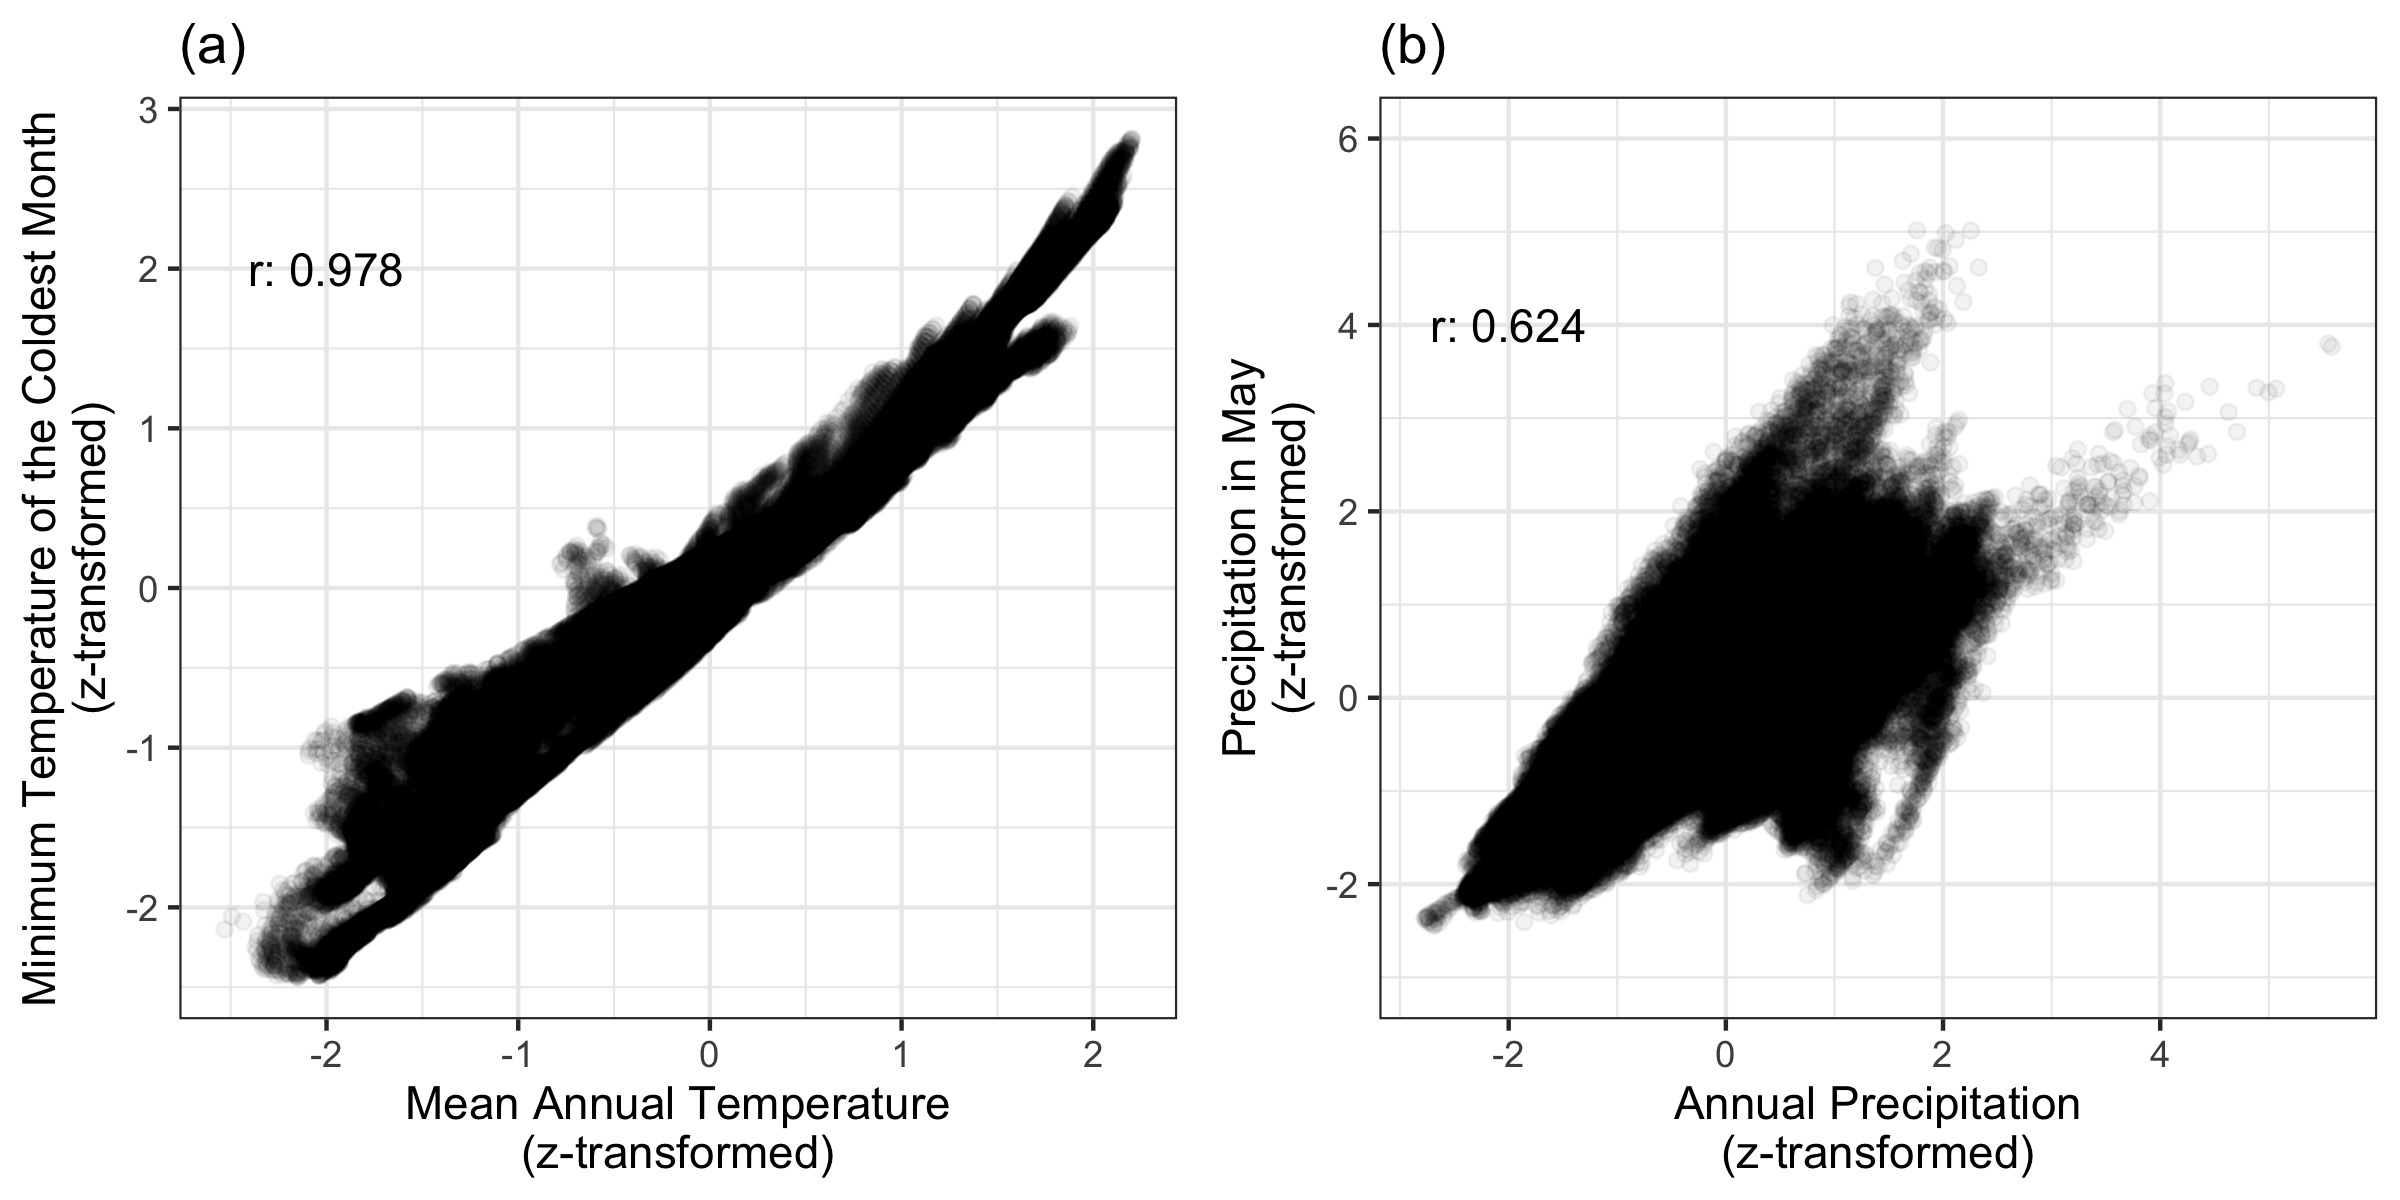
\includegraphics[width=\linewidth]{../../figs/Supp_CovScat.jpg}
    \caption{\label{fig:CovScatter} Scatter plots of z-transformed environmental covariates. (a) Mean Annual Temperature and Minimum Temperature of the Coldest Month, and (b) Annual Precipitation and Precipitation in May. The more general variables are highly correlated with the more specific variables across the eastern United States at a 5x5km resolution. The true demographic rates were related to the more specific variables, while the more general were used in the \emph{incorrect covariates} modelling scenario.}
\end{figure}
\begin{figure}
    \centering
    \captionsetup{width=\linewidth}
    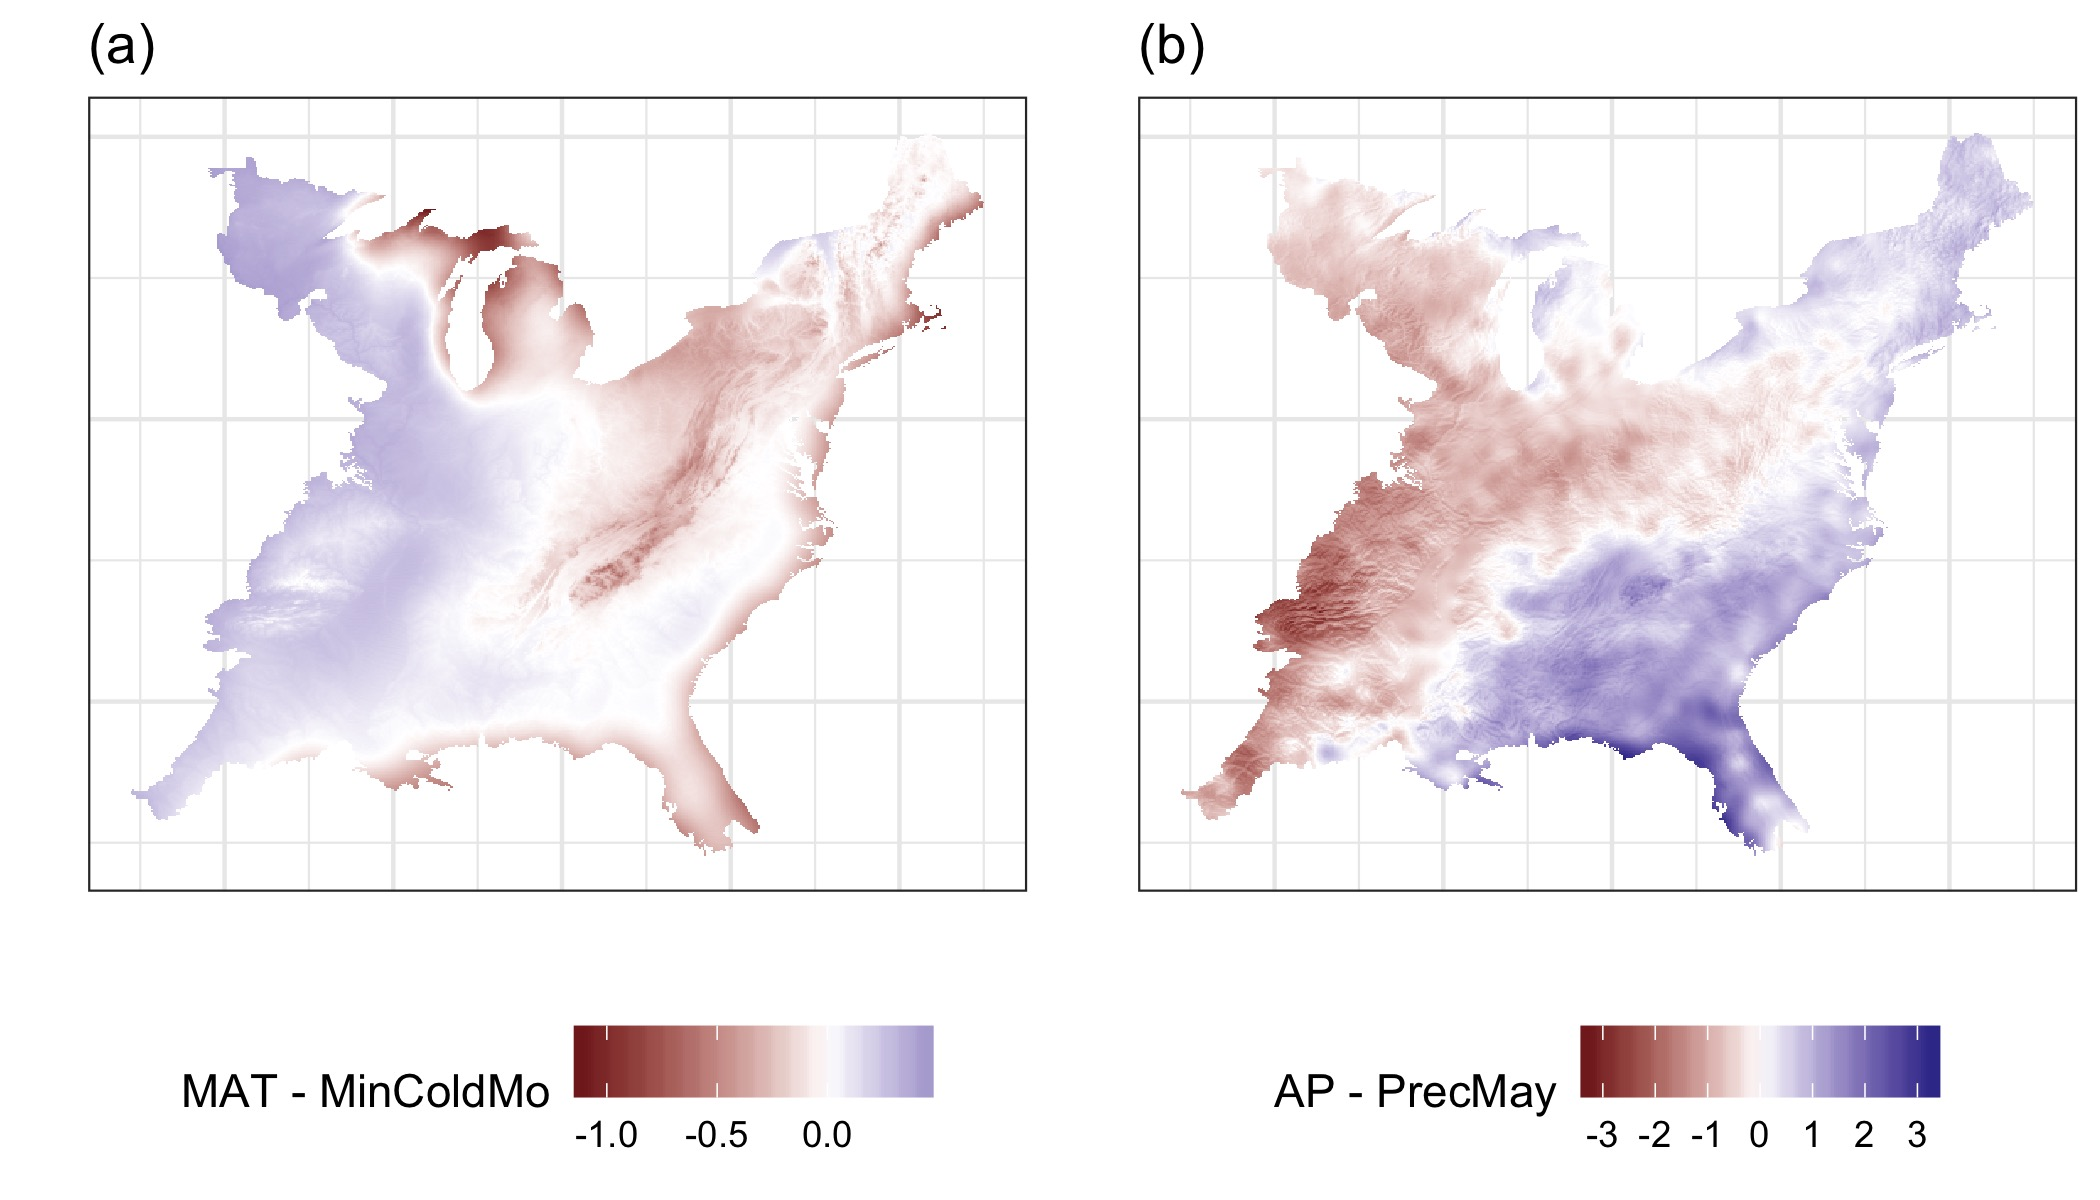
\includegraphics[width=\linewidth]{../../figs/Supp_CovMap.jpg}
    \caption{\label{fig:CovMap} Map of the difference between z-transformed environmental covariates. (a) Mean Annual Temperature and Minimum Temperature of the Coldest Month and (b) Annual Precipitation and Precipitation in May. Though highly correlated, the residuals show strong spatial patterning in each case.}
\end{figure}

\subsubsection{No seed bank}

This scenario applied only to the process-based SDMs. Seed bank dynamics
are difficult to quantify, and are poorly known in general relative to
other aspects of species' life cycles and ecology. A simple solution to
this problem is to assume negligible effects of the seed bank on
species' distributions or that any important effects are compensated for
by being implicitly included in estimates of related processes such as
direct germination. In this modelling scenario, we assume in each
process-based SDM that seed bank mortality is complete such that all
seedlings in year \(t\) originate from seeds produced in year \(t-1\).

\subsubsection{Under dispersal}

This scenario applied only to the process-based SDMs. Dispersal occurred
via both short distance and long distance processes, and both were
reduced in the \emph{under dispersal} scenario. Because two virtual
species had different dispersal strategies, where the shrub had more
effective short distance dispersal while the biennial relied more
heavily on long distance dispersal, we modified dispersal
proportionally. For long distance dispersal, the number of annual events
was decreased to 20\% of the true value. For short distance dispersal,
the rate of the exponential kernel was decreased by 50\%. Consequently,
the total number of seeds produced was unaffected, but chance dispersal
events to new regions were less likely, and seeds were more likely to be
dispersed to nearby cells within the short distance dispersal
neighborhood.

\subsubsection{Over dispersal}

This scenario applied only to the process-based SDMs. For the
\emph{over dispersal} scenario, the model mis-specification was reversed
compared to the \emph{under dispersal} scenario. Thus, for long distance
dispersal, the number of annual events was increased to 5 times the true
value. For short distance dispersal, the rate of the exponential kernel
was increased to 2 times the true value. Consequently, the total number
of seeds produced was unaffected, but chance dispersal events to new
regions were more likely, and cells toward the periphery of the short
distance dispersal neighborhood were more likely to receive seeds.

\begin{center}\rule{0.5\linewidth}{\linethickness}\end{center}

\section{References}

Allen, J. M., \& Bradley, B. A. (2016). Out of the weeds? Reduced plant
invasion risk with climate change in the continental United States.
Biological Conservation, 203(November), 306--312.
\url{https://doi.org/10.1016/j.biocon.2016.09.015}

Easterling, M. R., Ellner, S. P., \& Dixon, P. M. (2000). Size-specific
sensitivity: Applying a new structured population model. Ecology, 81(3),
694--708.
\url{https://doi.org/10.1890/0012-9658(2000)081\%5B0694:SSSAAN\%5D2.0.CO;2}

Ellner, S. P., \& Rees, M. (2006). Integral Projection Models for
Species with Complex Demography. The American Naturalist, 167(3),
410--428. \url{https://doi.org/10.1086/499438}

Manson, S., Schroeder, J., Van Riper, D., \& Ruggles, S. (2017). IPUMS
National Historical Geographic Information System: Version 12.0
{[}Database{]}. \url{https://doi.org/http://doi.org/10.18128/D050.V12.0}

Merow, C., Dahlgren, J. P., Metcalf, C. J. E., Childs, D. Z., Evans, M.
E. K., Jongejans, E., \ldots{} Mcmahon, S. M. (2014). Advancing
population ecology with integral projection models: A practical guide.
Methods in Ecology and Evolution, 5(2), 99--110.
\url{https://doi.org/10.1111/2041-210X.12146}

Merow, C., Bois, S. T., Allen, J. M., Xie, Y., \& Silander, J. A.
(2017). Climate change both facilitates and inhibits invasive plant
ranges in New England. Proceedings of the National Academy of Sciences,
114(16), E3276--E3284. \url{https://doi.org/10.1073/pnas.1609633114}

Szewczyk, T. M., Lee, T., Ducey, M. J., Aiello-Lammens, M. E., Bibaud,
H., \& Allen, J. M. (2019). Local management in a regional context :
Simulations with process-based species distribution models. Ecological
Modelling, 413(August), 108827.
\url{https://doi.org/10.1016/j.ecolmodel.2019.108827}

U.S. Census Bureau. (2017). 2017 TIGER/Line Shapefiles Technical
Documentation. Retrieved from
\url{https://www.census.gov/geo/maps-data/data/pdfs/tiger/tgrshp2012/TGRSHP2012_TechDoc.pdf}


\end{document}
